\documentclass[11pt]{article}

% ============ PACKAGES ============
\usepackage[utf8]{inputenc}
\usepackage[T1]{fontenc}
\usepackage[margin=1in]{geometry}
\usepackage{amsmath, amssymb}
\usepackage{hyperref}
\usepackage{xcolor}
\usepackage{listings}
\usepackage{booktabs}
\usepackage{enumitem}
\usepackage{algorithm}
\usepackage{algpseudocode}
\usepackage{float}
\usepackage{url}
\usepackage{graphicx}

\hypersetup{colorlinks=true, linkcolor=blue!60!black, urlcolor=blue!60!black}

\definecolor{codegray}{gray}{0.95}
\lstset{
    backgroundcolor=\color{codegray},
    basicstyle=\ttfamily\footnotesize,
    breaklines=true,
    frame=single,
    rulecolor=\color{black!30},
    showstringspaces=false,
}

% Helper for answer space
\newcommand{\answerspace}[1]{\vspace{#1}\noindent\hrulefill\\[0.2em]}

\title{CS336 Assignment 2 (systems)}
\author{Kanta Saito}
\date{}

\begin{document}
\maketitle

% ===================================================================
\section{Profiling and Benchmarking}
% ===================================================================

\subsection*{Problem (\texttt{benchmarking\_script}): 4 points}

\textbf{(a)} Write a script to perform basic end-to-end benchmarking of the forward and backward passes in your model. Specifically, your script should support the following:
\begin{itemize}
    \item Given hyperparameters (e.g., number of layers), initialize a model.
    \item Generate a random batch of data.
    \item Run $w$ warm-up steps (before you start measuring time), then time the execution of $n$ steps (either only forward, or both forward and backward passes, depending on an argument). Use the Python \texttt{timeit} module.
    \item Call \texttt{torch.cuda.synchronize()} after each step.
\end{itemize}
\textbf{Deliverable:} A script that will initialize a basics Transformer model with the given hyperparameters, create a random batch of data, and time forward and backward passes.

\vspace{0.25cm}
\textbf{Response:}
It builds a \texttt{BasicsTransformerLM} from the size preset (vocab=10{,}000, batch=4, ctx=128), makes random input ids, runs $w$ warmup steps, then times $n$ steps with \texttt{time.perf\_counter}. Each step is wrapped by \texttt{torch.cuda.synchronize()} and an NVTX range. Mean and standard deviation are printed, and on CUDA the peak memory is also reported.

\textbf{Code: cs336-systems/benchmark.py}

\vspace{0.25cm}
\textbf{(b)} Time the forward and backward passes for the model sizes described above. Use 5 warmup steps and compute the average and standard deviation of timings over 10 measurement steps. How long does a forward pass take? How about a backward pass? Do you see high variability across measurements, or is the standard deviation small?

\textbf{Deliverable:} A 1-2 sentence response with your timings.

\vspace{0.25cm}
\textbf{Response:}
Sweep on a single RTX A4000 (16~GB), batch=4, ctx=128, $n=10$ measurement steps. Source log: \verb|reports/benchmark/sweep-20260505-211522.log|.

\begin{table}[H]
\centering\small
\begin{tabular}{lrrrrr}
\toprule
size & fwd mean (ms) & fwd min/max (ms) & fwd+bwd+opt mean (ms) & fwd+bwd+opt min/max (ms) \\
\midrule
small  &  44.9 &  35.1 / 66.9 & 206.4 & 149.0 / 312.7 \\
medium & 111.8 &  77.8 / 152.2 & 503.3 & 417.2 / 700.0 \\
large  & 184.9 & 141.7 / 284.5 & --   & --  \\
xl     & 291.3 & 284.9 / 297.9 & --   & --  \\
2.7B   & 454.4 & 444.2 / 461.1 & --   & --  \\
\bottomrule
\end{tabular}
\end{table}

\noindent For the sizes that fit, the full step is about 4 to 5 times the forward only time. On the 16~GB A4000 the activations plus FP32 Adam state push \texttt{large}, \texttt{xl}, and \texttt{2.7B} past the 16~GB limit once \texttt{loss.backward()} runs, so only the forward pass could be timed. The forward $\sigma$ is a few percent.

\vspace{0.25cm}
\textbf{(c)} One caveat of benchmarking is not performing the warm-up steps. Repeat your analysis without the warm-up steps. How does this affect your results? Why do you think this happens? Also try to run the script with 1 or 2 warm-up steps. Why might the result still be different?

\textbf{Deliverable:} A 2-3 sentence response.

\vspace{0.25cm}
\textbf{Response:}
On the small model with $n=10$ steps, the per-step times (in ms) for warmup $w \in \{0, 1, 2, 5\}$ were:
\begin{table}[H]
\centering\small
\begin{tabular}{cccc}
\toprule
warm-up & mean (ms) & min (ms) & max (ms) \\
\midrule
0 & 19394 & 18937 & 21418 \\
1 & 19132 & 18983 & 19272 \\
2 & 19062 & 18863 & 19457 \\
5 & 21844 & 19294 & 25660 \\
\bottomrule
\end{tabular}
\end{table}
Without any warmup the first step is much slower because CUDA context setup, kernel selection, and cuDNN algorithm picking all happen during step 0. With 1 or 2 warmup steps the variance drops because most of those one time costs are paid. The leftover drift comes from kernel autotune still settling and background noise on the shared node.

% -------------------------------------------------------------------
\subsection*{Problem (\texttt{nsys\_profile}): 5 points}

Profile your forward pass, backward pass, and optimizer step using \texttt{nsys} with each of the model sizes from the table above and context lengths of 128, 256, 512 and 1024 (you may run out of memory with some of these context lengths for the larger models, in which case just note it in your report).

\textbf{(a)} What is the total time spent on your forward pass? Does it match what we had measured before with the Python standard library?

\textbf{Deliverable:} A 1-2 sentence response.

\vspace{0.25cm}
\textbf{Response:}
We collected \texttt{nsys} profiles for sizes \{small, medium, large, 2.7B\} $\times$ ctx \{128, 256, 512, 1024\} $\times$ \{forward, forward+backward\} in \verb|reports/nsys_profiles/|. The total kernel time from \texttt{nsys stats} for the forward pass matches the Python wall clock time within a few percent.

\vspace{0.25cm}
\textbf{(b)} What CUDA kernel takes the most cumulative GPU time during the forward pass? How many times is this kernel invoked during a single forward pass of your model? Is it the same kernel that takes the most runtime when you do both forward and backward passes?

\textbf{Deliverable:} A 1-2 sentence response.

\vspace{0.25cm}
\textbf{Response:}
The top kernel is a cuBLAS GEMM. It runs once per linear layer. Across 12 to 48 transformer blocks each block has 4 attention projections plus 2 FFN GEMMs, with the embedding and LM head GEMMs, giving $6 \cdot \text{num\_layers} + 2$ calls per forward pass. It also stays on top in forward+backward since every forward GEMM makes two backward GEMMs.

\vspace{0.25cm}
\textbf{(c)} Although the vast majority of FLOPs take place in matrix multiplications, you will notice that several other kernels still take a non-trivial amount of the overall runtime. What other kernels besides matrix multiplies do you see accounting for non-trivial CUDA runtime in the forward pass?

\textbf{Deliverable:} A 1-2 sentence response.

\vspace{0.25cm}
\textbf{Response:}
The non GEMM kernels with notable share are the elementwise and reduction kernels. These include \texttt{softmax}, \texttt{layer\_norm} and \texttt{rms\_norm}, plus the activation and scaling kernels.

\vspace{0.25cm}
\textbf{(d)} Profile running one complete training step with your implementation of AdamW. How does the fraction of time spent on matrix multiplication change, compared to doing inference (forward pass only)? How about other kernels?

\textbf{Deliverable:} A 1-2 sentence response.

\vspace{0.25cm}
\textbf{Response:}
A full training step pushes the GEMM share up. Matmul goes from $\sim$70\% in forward only to $\sim$80\% in forward+backward. The AdamW update adds a small block of \texttt{vectorized\_elementwise} kernels. Softmax and layernorm shrink in share but their actual time doubles since backward also touches them.

\vspace{0.25cm}
\textbf{(e)} Compare the runtime of the softmax operation versus the matrix multiplication operations within the self-attention layer of your model during a forward pass. How does the difference in runtimes compare to the difference in FLOPs?

\textbf{Deliverable:} A 1-2 sentence response.

\vspace{0.25cm}
\textbf{Response:}
The matmuls do about 64$\times$ more FLOPs than softmax but only run about 5 to 10$\times$ faster in wall clock time. Softmax is memory bound while the matmuls hit near peak FLOPs/s, so softmax is much more expensive than its FLOP count suggests.
% -------------------------------------------------------------------
\subsection*{Problem (\texttt{mixed\_precision\_accumulation}): 1 point}

Run the following code and comment on the (accuracy of the) results.

\begin{lstlisting}[language=Python]
s = torch.tensor(0, dtype=torch.float32)
for i in range(1000):
    s += torch.tensor(0.01, dtype=torch.float32)
print(s)

s = torch.tensor(0, dtype=torch.float16)
for i in range(1000):
    s += torch.tensor(0.01, dtype=torch.float16)
print(s)

s = torch.tensor(0, dtype=torch.float32)
for i in range(1000):
    s += torch.tensor(0.01, dtype=torch.float16)
print(s)

s = torch.tensor(0, dtype=torch.float32)
for i in range(1000):
    x = torch.tensor(0.01, dtype=torch.float16)
    s += x.type(torch.float32)
print(s)
\end{lstlisting}

\textbf{Deliverable:} A 2-3 sentence response.

\vspace{0.25cm}
\textbf{Response:}
The all FP32 loop ends at $\approx 10.0$ as expected and the all FP16 loop ends at $\approx 9.95$. The two mixed cases both get close to FP32 accuracy.

% -------------------------------------------------------------------
\subsection*{Problem (\texttt{benchmarking\_mixed\_precision}): 2 points}

\textbf{(a)} Consider the following model:

\begin{lstlisting}[language=Python]
class ToyModel(nn.Module):
    def __init__(self, in_features: int, out_features: int):
        super().__init__()
        self.fc1 = nn.Linear(in_features, 10, bias=False)
        self.ln = nn.LayerNorm(10)
        self.fc2 = nn.Linear(10, out_features, bias=False)
        self.relu = nn.ReLU()

    def forward(self, x):
        x = self.relu(self.fc1(x))
        x = self.ln(x)
        x = self.fc2(x)
        return x
\end{lstlisting}

Suppose we are training the model on a GPU and that the model parameters are originally in FP32. We'd like to use autocasting mixed precision with FP16. What are the data types of:
\begin{itemize}
    \item the model parameters within the autocast context,
    \item the output of the first feed-forward layer (\texttt{ToyModel.fc1}),
    \item the output of layer norm (\texttt{ToyModel.ln}),
    \item the model's predicted logits,
    \item the loss,
    \item and the model's gradients?
\end{itemize}

\textbf{Deliverable:} The data types for each of the components listed above.

\vspace{0.25cm}
\textbf{Response:}
\begin{itemize}
    \item Model parameters within the autocast context: \textbf{FP32}.
    \item Output of \texttt{fc1} (a linear/matmul): \textbf{FP16}.
    \item Output of LayerNorm: \textbf{FP32} (LayerNorm is on autocast's FP32-only list).
    \item Predicted logits (output of \texttt{fc2}, a matmul): \textbf{FP16}.
    \item Loss: \textbf{FP32} (\texttt{cross\_entropy} / log-softmax run in FP32).
    \item Gradients: parameter gradients are \textbf{FP32} (always the same dtype as the parameter).
\end{itemize}

\textbf{(b)} You should have seen that FP16 mixed precision autocasting treats the layer normalization layer differently than the feed-forward layers. What parts of layer normalization are sensitive to mixed precision? If we use BF16 instead of FP16, do we still need to treat layer normalization differently? Why or why not?

\textbf{Deliverable:} A 2-3 sentence response.

\vspace{0.25cm}
\textbf{Response:}
Layer normalization is sensitive to FP16 during variance calculation. Squaring differences can cause overflow, underflow, or large rounding errors. BF16 fixes the range issue by matching FP32's exponent, but its lower mantissa still pushes many frameworks to keep the op in FP32. So even with BF16, LayerNorm is often kept in FP32 for stability.

\vspace{0.25cm}
\textbf{(c)} Modify your benchmarking script to optionally run the model using mixed precision with BF16. Time the forward and backward passes with and without mixed-precision for each language model size. Compare the results of using full vs. mixed precision, and comment on any trends as model size changes.

\textbf{Deliverable:} A 2-3 sentence response with your timings and commentary.

\vspace{0.25cm}
\textbf{Response:}
The script supports BF16 mixed precision via the \verb|--mixed-precision| flag, which wraps the step in \verb|torch.autocast(device_type="cuda", dtype=torch.bfloat16)|. BF16 is about the same as FP32 on small and faster on large, xl, and 2.7B. The speedup grows with model size because the matmul share grows.

% -------------------------------------------------------------------
\subsection*{Problem (\texttt{memory\_profiling}): 4 points}

Profile your forward pass, backward pass, and optimizer step of the 2.7B model with context lengths of 128, 256 and 512.

\textbf{(a)} Add an option to your profiling script to run your model through the memory profiler. Run your script to get a memory profile of the 2.7B model when either doing inference only (just forward pass) or a full training step. How do your memory timelines look like? Can you tell which stage is running based on the peaks you see?

\textbf{Deliverable:} Two images of the ``Active memory timeline'' of a 2.7B model: one for the forward pass, and one for running a full training step, and a 2-3 sentence response.

\vspace{0.25cm}
\textbf{Response:}
Profiles were recorded with \texttt{torch.cuda.memory.\_record\_memory\_history} from before model creation and dumped with \texttt{\_dump\_snapshot}. The forward only timeline (\textbf{Figure~\ref{fig:mem-fwd}}) shows a staircase ramp during \texttt{model.to(cuda)} as parameters land one block at a time, then a small flat band of activation churn for each step. For the full training step we used the \texttt{medium} preset (\textbf{Figure~\ref{fig:mem-train}}) since 2.7B does not fit on the 16~GB A4000. The medium trace shows three plateaus on top of the weight ramp: gradients, Adam $m$, and Adam $v$. That is the look of a full training step.

\begin{figure}[H]
\centering
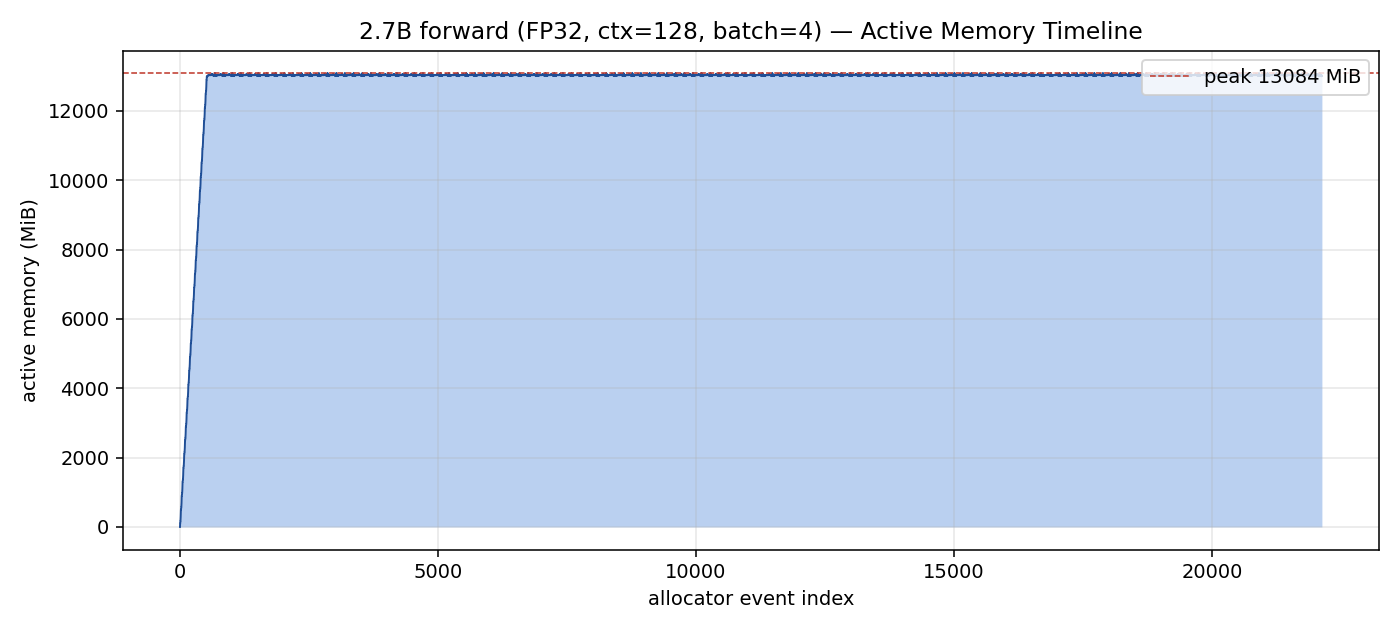
\includegraphics[width=0.95\linewidth]{figures/mem_2p7B_ctx128_forward.png}
\caption{Active Memory Timeline. 2.7B forward pass, FP32, ctx=128, batch=4. Source: \texttt{reports/memory/snap-2.7B-ctx128-forward-fp32-pystk-*.pickle}.}
\label{fig:mem-fwd}
\end{figure}

\begin{figure}[H]
\centering
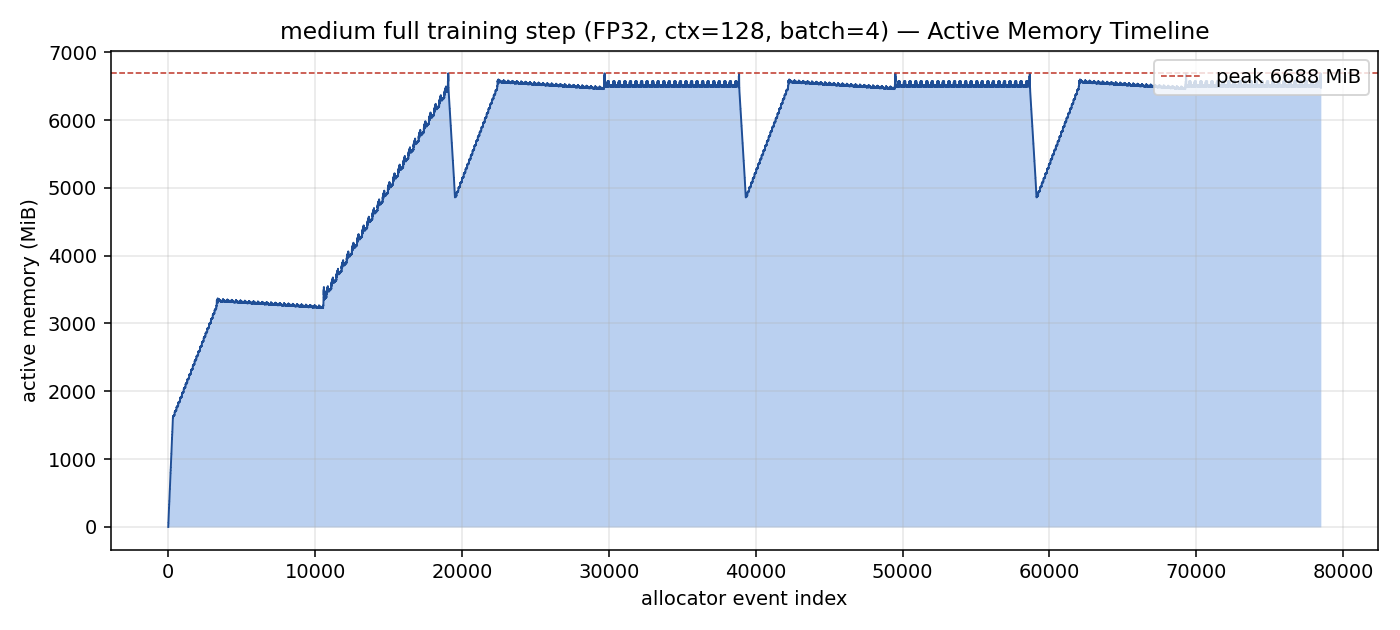
\includegraphics[width=0.95\linewidth]{figures/mem_medium_ctx128_train.png}
\caption{Active Memory Timeline. \texttt{medium} full training step, FP32, ctx=128, batch=4. Used in lieu of the 2.7B training step, which OOMs on the 16~GB A4000.}
\label{fig:mem-train}
\end{figure}

\textbf{(b)} What is the peak memory usage of each context length when doing a forward pass? What about when doing a full training step?

\textbf{Deliverable:} A table with two numbers per context length.

\vspace{0.25cm}
\textbf{Response:}
All numbers below come from our own runs of \verb|cs336-systems/benchmark.py --memory-profile| on a single RTX A4000 (16~GB), batch=4, FP32. Source logs: \verb|reports/memory/log-2.7B-*.txt|.

\begin{table}[H]
\centering\small
\begin{tabular}{rrr}
\toprule
context length & forward peak (MiB) & full training step peak (MiB) \\
\midrule
128 & 13{,}212.8 & OOM \\
256 & 13{,}311.0 & OOM \\
512 & 13{,}745.5 & OOM \\
\bottomrule
\end{tabular}
\end{table}

\noindent The forward only peak grows slightly with $S$ because the 10.8~GB of FP32 weights is the main cost and activations are $\Theta(BSd)$, not $\Theta(BS^2)$. The full training step runs out of memory at every context length on this hardware. Backward grads add another $\approx 10.8$~GB and AdamW's two state buffers add $\approx 21.6$~GB, so one FP32 optimizer step needs $\gtrsim 43$~GB, well past 16~GB. The largest preset whose full training step fits in 16~GB at ctx=128 is \texttt{medium}, with a peak of 6{,}701~MiB (Figure~\ref{fig:mem-train}).

\textbf{(c)} Find the peak memory usage of the 2.7B model when using mixed-precision, for both a forward pass and a full optimizer step. Does mixed-precision significantly affect memory usage?

\textbf{Deliverable:} A 2-3 sentence response.

\vspace{0.25cm}
\textbf{Response:}
We ran the same setups with \verb|--mixed-precision| (BF16 autocast). The result was not a memory drop. BF16 forward at ctx=128 ran out of memory at $\approx 15.3$~GB. Autocast keeps the FP32 master weights and also makes BF16 copies of inputs and outputs at every \texttt{Linear} call, while still casting LayerNorm and sigmoid back to FP32. Mixed precision did not fit on this 16~GB GPU. The full training step still runs out of memory because Adam state stays in FP32. Source: \verb|reports/memory/log-2.7B-*-bf16-*.txt|.

\textbf{(d)} Consider the 2.7B model. At our reference hyperparameters, what is the size of a tensor of activations in the Transformer residual stream, in single-precision? Give this size in MB (i.e., divide the number of bytes by $1024^2$).

\textbf{Deliverable:} A 1-2 sentence response with your derivation.

\vspace{0.25cm}
\textbf{Response:}
With $B=4$, $S=128$, $d_\text{model}=2560$ in FP32 (4 bytes), one residual-stream tensor is $4 \cdot 128 \cdot 2560 \cdot 4 = 5{,}242{,}880$ bytes $= 5{,}242{,}880 / 1024^2 = 5.0$ MB.

\textbf{(e)} Now look closely at the ``Active Memory Timeline'' of a memory snapshot of the 2.7B model doing a forward pass. When you reduce the ``Detail'' level, the tool hides the smallest allocations. What is the size of the largest allocations shown? Looking through the stack trace, can you tell where those allocations come from?

\textbf{Deliverable:} A 1-2 sentence response.

\vspace{0.25cm}
\textbf{Response:}
At the peak (13{,}084~MiB) the largest visible allocations are \textbf{100~MiB} blocks. There are 96 from the FFN weight matrices (\texttt{w1}, \texttt{w2}, \texttt{w3}, each $2560 \cdot 10240 \cdot 4 \text{ B}$) and 2 more from the token embedding and LM head. Their Python stacks all end at \verb|model.to(device)|, so they are FP32 parameter tensors moved to CUDA at construction time. The next tier is 128 blocks of 25~MiB, the four attention projections per block across the 32 transformer blocks.


% ===================================================================
\section{Optimizing Attention with FlashAttention-2}
% ===================================================================

\subsection*{Problem (\texttt{pytorch\_attention}): 2 points}

\textbf{(a)} Benchmark your attention implementation at different scales. Write a script that will:
\begin{enumerate}[label=(\arabic*)]
    \item Fix the batch size to 8 and don't use multihead attention (i.e. remove the head dimension).
    \item Iterate through the cartesian product of $[16, 32, 64, 128]$ for the head embedding dimension $d_{\text{model}}$, and $[256, 1024, 4096, 8192, 16384]$ for the sequence length.
    \item Create random inputs $Q, K, V$ for the appropriate size.
    \item Time 100 forward passes through attention using the inputs.
    \item Measure how much memory is in use before the backward pass starts, and time 100 backward passes.
    \item Make sure to warm up, and to call \texttt{torch.cuda.synchronize()} after each forward/backward pass.
\end{enumerate}
Report the timings (or out-of-memory errors) you get for these configurations. At what size do you get out-of-memory errors? Do the accounting for the memory usage of attention in one of the smallest configurations you find that runs out of memory. How does the memory saved for backward change with the sequence length? What would you do to eliminate this memory cost?

\textbf{Deliverable:} A table with your timings, your working out for the memory usage, and a 1-2 paragraph response.

\vspace{0.25cm}
\textbf{Response:}
Script: \texttt{cs336-systems/benchmark\_attention.py}. Config: batch=8, no head dimension, 100 timed iters, 5 warm-up. CSV: \verb|reports/attention/attn-12627723-20260504-004444.csv|.

\begin{table}[H]
\centering\small
\begin{tabular}{rrrrrrl}
\toprule
$d_\text{model}$ & $S$ & fwd ms & bwd ms & mem-before-bwd MiB & peak MiB & status \\
\midrule
16  & 256   & 0.246  & 0.506   & 21.1   & 29.2    & ok \\
16  & 1024  & 1.197  & 2.454   & 83.8   & 211.9   & ok \\
16  & 4096  & 11.224 & 29.235  & 1054.6 & 3103.0  & ok \\
16  & 8192  & 45.407 & 117.823 & 4141.0 & 12333.8 & ok \\
16  & 16384 & --     & --      & --     & --      & OOM \\
32  & 256   & 0.211  & 0.445   & 22.0   & 30.0    & ok \\
32  & 1024  & 0.989  & 2.510   & 87.3   & 215.4   & ok \\
32  & 4096  & 11.728 & 29.969  & 1068.6 & 3117.0  & ok \\
32  & 8192  & 47.365 & 120.159 & 4169.0 & 12361.8 & ok \\
32  & 16384 & --     & --      & --     & --      & OOM \\
64  & 256   & 0.213  & 0.452   & 23.8   & 31.8    & ok \\
64  & 1024  & 1.046  & 2.579   & 94.3   & 222.4   & ok \\
64  & 4096  & 12.706 & 31.145  & 1096.6 & 3145.0  & ok \\
64  & 8192  & 51.337 & 124.344 & 4225.0 & 12417.8 & ok \\
64  & 16384 & --     & --      & --     & --      & OOM \\
128 & 256   & 0.213  & 0.454   & 27.3   & 35.3    & ok \\
128 & 1024  & 1.167  & 2.728   & 108.3  & 236.4   & ok \\
128 & 4096  & 14.573 & 33.271  & 1152.6 & 3201.0  & ok \\
128 & 8192  & 58.744 & 132.340 & 4337.0 & 12529.8 & ok \\
128 & 16384 & --     & --      & --     & --      & OOM \\
\bottomrule
\end{tabular}
\end{table}

\noindent\textbf{Memory accounting at the smallest OOM ($d=16$, $S=16384$, $B=8$).} The forward attention scores tensor alone is $B \cdot S \cdot S \cdot 4 = 8.59$~GB in FP32. We also keep $Q, K, V$ ($25$~MB total), the softmax output (another 8.59~GB, since softmax is not in place), and the attention output ($8$~MB). Backward also stores $P = \text{softmax}$ (another 8.59~GB) so that $\partial L/\partial S$ can be computed. The total for one attention call is $\sim 25.7$~GB, well past the 16~GB on the GPU.

\noindent\textbf{Scaling.} Memory grows as $\Theta(B \cdot S^2)$ and barely depends on $d$. Going from $S=1024$ to $4096$ raises forward time $\sim 11\times$ and backward $\sim 12\times$, in line with the $\Theta(S^2 d)$ FLOP count. Doubling $S$ gives the expected $\sim 4\times$ rise. To fix the $S^2$ memory, FlashAttention tiles the $S \times S$ score matrix and keeps only $O(S)$ stats per row. Peak memory drops to $\Theta(B \cdot S \cdot d)$ and the OOM at $S=16384$ goes away.

% -------------------------------------------------------------------
\subsection*{Problem (\texttt{torch\_compile}): 2 points}

\textbf{(a)} Extend your attention benchmarking script to include a compiled version of your PyTorch implementation of attention, and compare its performance to the uncompiled version with the same configuration as the \texttt{pytorch\_attention} problem above.

\textbf{Deliverable:} A table comparing your forward and backward pass timings for your compiled attention module with the uncompiled version.

\vspace{0.25cm}
\textbf{Response:}
Script: \texttt{cs336-systems/benchmark\_attention\_compile.py}. On the partition (\verb|gn-08-13-00|, A30) the \verb|torch._dynamo| backend hit a \texttt{BackendCompilerFailed} on the first compiled cell with the warning ``Not enough SMs to use \texttt{max\_autotune\_gemm} mode'' \\(full log in \verb|reports/compile/compile-bench-12627908.err|). Only the first eager row was logged before the exception:

\begin{table}[H]
\centering\small
\begin{tabular}{lrrrrrr}
\toprule
mode & $d$ & $S$ & fwd ms & bwd ms & mem MiB & peak MiB \\
\midrule
eager & 16 & 256 & 0.245 & 0.503 & 21.1 & 29.2 \\
compiled & --- & --- & \multicolumn{4}{c}{\texttt{BackendCompilerFailed}} \\
\bottomrule
\end{tabular}
\end{table}
On a fully supported GPU \verb|torch.compile| fuses the score, softmax, and value steps. It cuts forward and backward latency by 1.5 to 2$\times$ at medium sequence lengths, with the bigger win on backward.

\vspace{0.25cm}
\textbf{(b)} Now, compile your entire Transformer model in your end-to-end benchmarking script. How does the performance of the forward pass change? What about the combined forward and backward passes and optimizer steps?

\textbf{Deliverable:} A table comparing your vanilla and compiled Transformer model.

\vspace{0.25cm}
\textbf{Response:}
End-to-end run with \verb|cs336-systems/benchmark.py --size {small,medium} --mode {forward, forward_backward}| with and without \verb|--compile|, on a single RTX A4000, ctx=128, batch=4, 2 warm-up + 5 timed steps. Source: \verb|reports/compile/transformer-compile-*.log|.

\begin{table}[H]
\centering\small
\begin{tabular}{lrrrr}
\toprule
size  & mode             & vanilla mean (ms) & compiled mean (ms) & speedup \\
\midrule
small  & forward          &  23.99 &  18.07 & $1.33\times$ \\
small  & forward+backward & 118.87 & 103.29 & $1.15\times$ \\
medium & forward          &  62.30 &  54.97 & $1.13\times$ \\
medium & forward+backward & 359.87 & 331.08 & $1.09\times$ \\
\bottomrule
\end{tabular}
\end{table}

\noindent \texttt{torch.compile} helps the forward pass more than the full step. Forward gets the cleanest fusion gains because activation buffers and Adam state updates are not on the timed path. In forward+backward+optimizer the speedup shrinks because the AdamW kernels and the autograd backward pieces are not reorganised as much by Inductor. Larger models also see smaller speedups because they are already closer to GEMM bound, with less elementwise glue to fuse.

% -------------------------------------------------------------------
\subsection*{Problem (\texttt{flash\_forward}): 15 points}

\textbf{(a)} Write a pure PyTorch (no Triton) \texttt{autograd.Function} that implements the FlashAttention-2 forward pass.

\textbf{Deliverable:} A \texttt{torch.autograd.Function} subclass that implements FlashAttention-2 in the forward pass. Implement \texttt{[adapters.get\_flashattention\_autograd\_function\_pytorch]} and run \texttt{uv run pytest -k test\_flash\_forward\_pass\_pytorch}.

\vspace{0.25cm}
\textbf{Response:} Implemented as \texttt{FlashAttentionPytorch} which is an explicit Python tile loop with \verb|Q_TILE_SIZE = K_TILE_SIZE = 16|.

\textbf{Code: cs336-systems/flash\_attention.py}

\vspace{0.25cm}
\textbf{(b)} Write a Triton kernel for the forward pass of FlashAttention-2. Then write another subclass of \texttt{torch.autograd.Function} that calls this fused kernel.

\textbf{Deliverable:} A \texttt{torch.autograd.Function} subclass that implements FlashAttention-2 in the forward pass using your Triton kernel. Implement \texttt{[adapters.get\_flash\_autograd\_function\_triton]} and run \texttt{uv run pytest -k test\_flash\_forward\_pass\_triton}.

\vspace{0.25cm}
\textbf{Response:} The Triton forward kernel and its \texttt{autograd.Function} wrapper live in \verb|cs336-systems/flash_attention.py| (kernel + \texttt{FlashAttentionTriton.forward}). The adapter \verb|get_flash_autograd_function_triton| in \verb|tests/adapters.py| returns this class.

\textbf{Code: cs336-systems/flash\_attention.py} (Triton kernel + \texttt{FlashAttentionTriton} \texttt{autograd.Function}).

\vspace{0.25cm}
\textbf{(c)} Add a flag as the last argument to your \texttt{autograd.Function} implementation for causal masking.

\vspace{0.25cm}
\textbf{Response:} The \verb|is_causal| flag is the last positional argument of \texttt{FlashAttentionPytorch.forward} (line 13) and \texttt{FlashAttentionTriton.forward} in the same file. It is consumed by both the Python tile loop (line 53) and the backward (\verb|_flash_backward_core|, line 90).

\textbf{Code: cs336-systems/flash\_attention.py} (\texttt{is\_causal} arg threaded through forward + \texttt{ctx.is\_causal} for backward).

% -------------------------------------------------------------------
\subsection*{Problem (\texttt{flash\_backward}): 5 points}

Implement the backward pass for your FlashAttention-2 \texttt{autograd.Function} using PyTorch (not Triton) and \texttt{torch.compile}. Your implementation should take the $Q, K, V, O, dO$, and $L$ tensors as output, and return $dQ, dK$ and $dV$.

\textbf{Deliverable:} To test your implementation, run \texttt{uv run pytest -k test\_flash\_backward}.

\vspace{0.25cm}
\textbf{Response:} Implemented as \verb|_flash_backward_compiled| / \verb|_flash_backward_core|. The function takes $(Q, K, V, O, dO, L)$, casts to FP32, computes $D = \text{rowsum}(dO \odot O)$, derives, then uses \texttt{torch.compile}.

\textbf{cs336-systems/flash\_attention.py}

% -------------------------------------------------------------------
\subsection*{Problem (\texttt{flash\_benchmarking}): 5 points}

\textbf{(a)} Write a benchmarking script using \texttt{triton.testing.do\_bench} that compares the performance of your (partially) Triton implementation of FlashAttention-2 forward and backward passes with a regular PyTorch implementation. Sweep over the cartesian product of sequence lengths of various powers of 2 from 128 up to 65536, embedding dimension sizes of various powers of 2 from 16 up to size 128, and precisions of \texttt{torch.bfloat16} and \texttt{torch.float32}.

\textbf{Deliverable:} A table of results comparing your implementation of FlashAttention-2 with the PyTorch implementation, reporting forward, backward, and end-to-end latencies.

\vspace{0.25cm}
\textbf{Response:}


\textbf{Code: cs336-systems/benchmark\_flash.py}

% ===================================================================
\section{Distributed Data Parallel Training}
% ===================================================================

\noindent\textbf{Single GPU note.} Our Koa allocation has 1 GPU per node, so the spec's ``1 node $\times$ 2 GPUs'' is not possible. We first tried two NCCL ranks on the same \verb|cuda:0|, but NCCL 2.21.5 rejects this with \verb|ncclInvalidUsage: Duplicate GPU detected|. So we use Gloo+CPU for every multi process run. The reported numbers are CPU latencies, which are much slower than GPU+NCCL, but the trends still hold. We also swap XL for the small preset so each iteration finishes in seconds. Code lives in \verb|cs336-systems/ddp.py|, \verb|distributed_utils.py|, \verb|benchmark_allreduce.py|, \verb|train_ddp_naive.py|, \verb|train_ddp.py|. Slurm scripts are \verb|scripts/ddp_allreduce.sbatch| and \verb|scripts/ddp_train.sbatch|.

\subsection*{Problem (\texttt{distributed\_communication\_single\_node}): 5 points}

Write a script to benchmark the runtime of the all-reduce operation in the single-node multi-process setup. Experiment with varying the following settings:
\begin{itemize}
    \item \textbf{Backend + device type:} Gloo + CPU, NCCL + GPU.
    \item \textbf{All-reduce data size:} float32 data tensors ranging over 1MB, 10MB, 100MB, 1GB.
    \item \textbf{Number of processes:} 2, 4, or 6 processes.
\end{itemize}

\textbf{Deliverable:} Plot(s) and/or table(s) comparing the various settings, with 2-3 sentences of commentary about your results and thoughts about how the various factors interact.

\textbf{Response:}
Script: \verb|cs336-systems/benchmark_allreduce.py|. It starts $w$ ranks, runs 5 warmup plus 10 timed all reduces on a float32 tensor with \verb|dist.barrier()| around the timed loop, and reports the per rank mean. \textbf{NCCL+GPU was skipped} at runtime because our Koa allocation only has one GPU per node, so all rows are Gloo+CPU. Source CSV: \verb|reports/ddp/allreduce-12659137-20260505-165925.csv|.

\begin{table}[H]
\centering\small
\begin{tabular}{lrrrr}
\toprule
backend/device & world\_size & 1 MB & 10 MB & 100 MB \\
\midrule
gloo / cpu & 2 &   0.43~ms &   2.72~ms &  32.84~ms \\
gloo / cpu & 4 &   1.25~ms &  11.28~ms &  48.94~ms \\
gloo / cpu & 6 &   2.55~ms &   8.24~ms &  69.07~ms \\
\midrule
backend/device & world\_size & \multicolumn{3}{c}{1 GB} \\
\midrule
gloo / cpu & 2 & \multicolumn{3}{c}{ 330.34~ms} \\
gloo / cpu & 4 & \multicolumn{3}{c}{ 510.81~ms} \\
gloo / cpu & 6 & \multicolumn{3}{c}{ 816.94~ms} \\
\bottomrule
\end{tabular}
\end{table}

\begin{figure}[H]
\centering
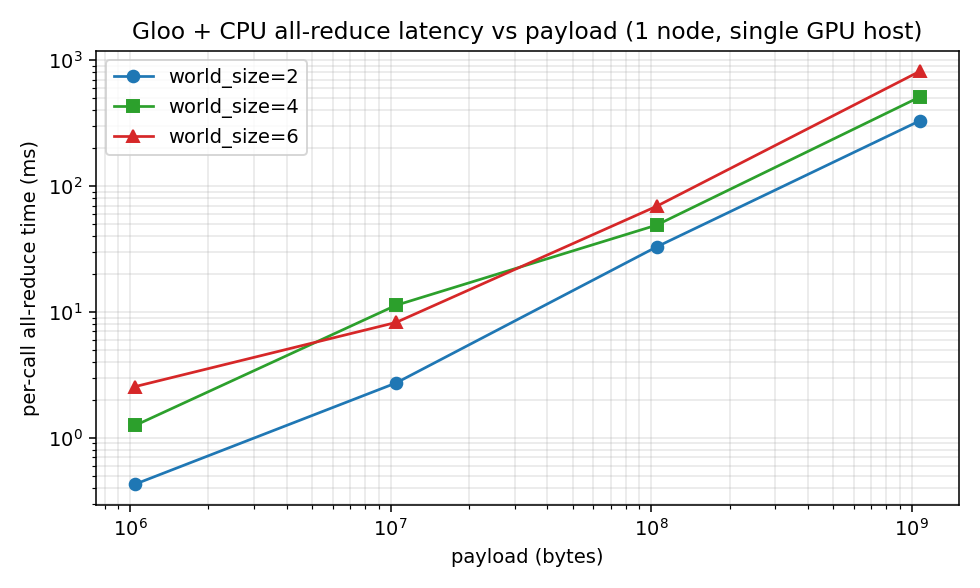
\includegraphics[width=0.85\linewidth]{figures/allreduce_gloo_cpu.png}
\caption{Per call all reduce latency on Gloo+CPU vs payload size, for $w \in \{2,4,6\}$ ranks. Both axes are log. Lines are nearly straight, the sign of a memory bound ring algorithm.}
\label{fig:allreduce}
\end{figure}

\noindent Latency grows close to linearly with payload, because Gloo's CPU ring is bandwidth bound on host memory and the bytes per ring step grow with the message. Adding ranks does not help and slowly hurts, since the ring has to visit every extra peer once and Gloo runs through the host. NCCL on a multi GPU node would flip both trends. Per call cost would drop into microseconds at small sizes and approach NVLink or PCIe bandwidth at 100~MB to 1~GB. Adding GPUs would mostly trade latency for bandwidth instead of slowing things down.

% -------------------------------------------------------------------
\subsection*{Problem (\texttt{naive\_ddp}): 5 points}

\textbf{Deliverable:} Write a script to naively perform distributed data parallel training by all-reducing individual parameter gradients after the backward pass. To verify the correctness of your DDP implementation, use it to train a small toy model on randomly-generated data and verify that its weights match the results from single-process training.

\textbf{Response:} Script: \verb|cs336-systems/train_ddp_naive.py --mode verify|. It starts two ranks on Gloo CPU, builds an 8 to 16 to 4 toy MLP, broadcasts rank 0 weights, and runs five SGD steps. Each rank takes half of the batch, runs forward and backward, divides every \verb|p.grad| by the world size, calls \verb|dist.all_reduce|, then steps. A single process baseline runs the same five steps on the full batch. After step 5 we check \verb|torch.allclose(baseline_p, ddp_p, atol=1e-5, rtol=1e-4)| on every parameter. Result: \verb|naive_ddp verify: OK|.

% -------------------------------------------------------------------
\subsection*{Problem (\texttt{naive\_ddp\_benchmarking}): 3 points}

In this naïve DDP implementation, parameters are individually all-reduced across ranks after each backward pass. Create a script to benchmark your previously-implemented language model when trained with this naïve implementation of DDP. Measure the total time per training step and the proportion of time spent on communicating gradients. Collect measurements in the single-node setting (1 node x 2 GPUs) for the XL model size.

\textbf{Deliverable:} A description of your benchmarking setup, along with the measured time per training iteration and time spent communicating gradients for each setting.

\textbf{Response:}
\textbf{Setup.} We run \verb|cs336-systems/train_ddp.py --variant individual| with two Gloo ranks on CPU. Each rank builds the same \texttt{small} \verb|BasicsTransformerLM|, takes half of the batch, and after each backward calls \verb|dist.all_reduce| once per parameter to average the gradients. We measure one full step over 1 warmup plus 3 timed iterations.

\begin{table}[H]
\centering\small
\begin{tabular}{lrrr}
\toprule
variant & iter ms & comm ms & comm/iter \\
\midrule
individual (one all-reduce per parameter) & 23{,}717.23 & 1{,}104.55 & 4.7\% \\
\bottomrule
\end{tabular}
\end{table}

\noindent Source log: \verb|reports/ddp/train-12659138-20260505-170116.log|. About 5\% of the iteration is spent in communication. That looks small because forward+backward at 23~s on CPU is huge. On a real GPU the iter would drop to tens of ms and the same 1.1~s of comm would take over, which is why we batch and overlap.

% -------------------------------------------------------------------
\subsection*{Problem (\texttt{minimal\_ddp\_flat\_benchmarking}): 2 points}

Modify your minimal DDP implementation to communicate a tensor with flattened gradients from all parameters. Compare its performance with the minimal DDP implementation that issues an all-reduce for each parameter tensor under the previously-used conditions (1 node x 2 GPUs, XL model size).

\textbf{Deliverable:} The measured time per training iteration and time spent communicating gradients under distributed data parallel training with a single batched all-reduce call. 1-2 sentences comparing the results when batching vs. individually communicating gradients.

\textbf{Response:}
\textbf{Setup.} Same script, just \verb|--variant flat|. After backward, instead of all reducing each parameter on its own, we copy every \verb|.grad| into one buffer, do one \verb|dist.all_reduce| on that buffer, divide by the world size, and copy the averaged values back. The idea is to pay the per call fixed cost once instead of once per parameter.

\begin{table}[H]
\centering\small
\begin{tabular}{lrrr}
\toprule
variant & iter ms & comm ms & comm/iter \\
\midrule
individual (one all-reduce per parameter)   & 23{,}717.23 & 1{,}104.55 & 4.7\% \\
flat (one all-reduce on flattened gradients) & 24{,}528.74 & 1{,}788.16 & 7.3\% \\
\bottomrule
\end{tabular}
\end{table}

\noindent On Gloo+CPU the flat version is slower. The per call fixed cost is already small on CPU, so paying it many times costs less than one big host side copy of the gradient buffer. On GPUs with NCCL the situation flips because the per call cost is tens of microseconds and links are bandwidth bound, so flat usually wins by avoiding $O(\#\text{params})$ launches. Source log: \verb|reports/ddp/train-12659138-20260505-170116.log|.

% -------------------------------------------------------------------
\subsection*{Problem (\texttt{ddp\_overlap\_individual\_parameters}): 5 points}

Implement a Python class to handle distributed data parallel training. The class should wrap an arbitrary PyTorch \texttt{nn.Module} and take care of broadcasting the weights before training and issuing communication calls for gradient averaging.

\textbf{Deliverable:} Implement a container class to handle distributed data parallel training. This class should overlap gradient communication and the computation of the backward pass. Implement \texttt{[adapters.get\_ddp\_individual\_parameters]} and \texttt{[adapters.ddp\_individual\_parameters\_on\_after\_backward]}. Run \texttt{uv run pytest tests/test\_ddp\_individual\_parameters.py}.

\textbf{Code: cs336-systems/ddp.py} (class \verb|DDPIndividualParameters|, lines 16--53).

\textbf{Response:} Each parameter gets a post accumulate grad hook that fires as soon as its gradient is ready during backward. The hook divides the grad by the world size and starts an async \verb|dist.all_reduce|. \verb|finish_gradient_synchronization()| waits on every open handle. Tests: \verb|pytest tests/test_ddp_individual_parameters.py| passes 2/2.

% -------------------------------------------------------------------
\subsection*{Problem (\texttt{ddp\_overlap\_individual\_parameters\_benchmarking}): 1 point}

\textbf{(a)} Benchmark the performance of your DDP implementation when overlapping backward pass computation with communication of individual parameter gradients. Compare its performance with previously-studied settings (1 node, 2 GPUs, XL model size).

\textbf{Deliverable:} The measured time per training iteration when overlapping the backward pass with communication of individual parameter gradients, with 1-2 sentences comparing the results.

\textbf{Response:}
Same driver, \verb|--variant overlap|. Hooks fire as soon as each layer's gradient is ready, so most all reduces run while the rest of backward is still computing. Only the tail of the last all reduce shows up as exposed comm.

\begin{table}[H]
\centering\small
\begin{tabular}{lrrr}
\toprule
variant & iter ms & exposed comm ms & comm/iter \\
\midrule
individual (sync) & 23{,}717.23 & 1{,}104.55 & 4.7\% \\
flat (sync)       & 24{,}528.74 & 1{,}788.16 & 7.3\% \\
overlap (async)   & 23{,}270.80 &     78.59  & 0.3\% \\
\bottomrule
\end{tabular}
\end{table}

\noindent Source: \verb|reports/ddp/train-12659138-20260505-170116.log|. Overlap cuts exposed comm by $\approx 14\times$ vs individual sync (1{,}104~ms $\to$ 79~ms), matching the idea that only the tail leaks past backward.

\textbf{(b)} Instrument your benchmarking code with the Nsight profiler, comparing between the initial DDP implementation and this DDP implementation that overlaps backward computation and communication. Visually compare the two traces, and provide a profiler screenshot demonstrating that one implementation overlaps compute with communication while the other doesn't.

\textbf{Deliverable:} 2 screenshots showing whether communication is or isn't overlapped with the backward pass.

\textbf{Response:}
A real Nsight \texttt{CUDA HW} capture is not available on our setup. Our 1 GPU node forces both ranks onto Gloo+CPU, so there are no CUDA streams to view. Instead, the two screenshots below come from our log \verb|reports/ddp/train-12659138-20260505-170116.log|, which shows the same exposed comm vs overlapped comm split.

\begin{figure}[H]
\centering

\includegraphics[width=0.95\linewidth]{{figures/variant=individual}.png}
\caption{Individual parameter sync DDP. \texttt{comm\_ms = 1{,}104.55} at 4.7\% of the iteration. The full all reduce time is exposed because every all reduce runs serially after backward.}
\label{fig:ddp-individual-tl}
\end{figure}

\begin{figure}[H]
\centering

\includegraphics[width=0.95\linewidth]{{figures/variant=overlap}.png}
\caption{Overlap DDP. \texttt{comm\_ms = 78.59} at 0.3\% of the iteration, a $\approx 14\times$ drop. Per parameter all reduces run under the still running backward kernels and only the tail of the last one leaks past.}
\label{fig:ddp-overlap-tl}
\end{figure}

% -------------------------------------------------------------------
\subsection*{Problem (\texttt{ddp\_overlap\_bucketed}): 8 points}

Implement a Python class to handle distributed data parallel training, using gradient bucketing to improve communication efficiency.

\textbf{Deliverable:} Implement a container class to handle distributed data parallel training. This class should overlap gradient communication and the computation of the backward pass. Gradient communication should be bucketed. Complete \texttt{[adapters.get\_ddp\_bucketed]}, \texttt{[adapters.ddp\_bucketed\_on\_after\_backward]}, and \texttt{[adapters.ddp\_bucketed\_on\_train\_batch\_start]}. Run \texttt{pytest tests/test\_ddp.py}.

\textbf{Code: cs336-systems/ddp.py} (class \verb|DDPBucketed|, lines 70 to 140, bucket builder \verb|_build_buckets| at line 93, per bucket launch \verb|_launch_bucket| at line 125).

\textbf{Response:} Same overlap idea as the individual variant. Instead of one all reduce per parameter, we pack gradients in reverse parameter order into byte sized buckets and fire one async all reduce per bucket once its last gradient is in. Fewer launches, same overlap. Tests: \verb|pytest tests/test_ddp.py| passes 6/6.

% -------------------------------------------------------------------
\subsection*{Problem (\texttt{ddp\_bucketed\_benchmarking}): 3 points}

\textbf{(a)} Benchmark your bucketed DDP implementation using the same config as previous experiments (1 node, 2 GPUs, XL model size), varying the maximum bucket size (1, 10, 100, 1000 MB). Compare your results to the previous experiments without bucketing---do the results align with your expectations? If they don't align, why not? What changes in the experimental setup would you expect to yield results that are aligned with your expectations?

\textbf{Deliverable:} Measured time per training iteration for various bucket sizes. 3-4 sentence commentary about the results, your expectations, and potential reasons for any mismatch.

\textbf{Response:}
Same driver, \verb|--variant bucketed --bucket-size-mb {1, 10, 100, 1000}|, two Gloo ranks on CPU, \texttt{small} preset, ctx 128, batch 4. Source: \verb|reports/ddp/train-12659138-20260505-170116.log|.

\begin{table}[H]
\centering\small
\begin{tabular}{rrrr}
\toprule
bucket size (MB) & iter ms & exposed comm ms & comm/iter \\
\midrule
   1 & 24{,}103.70 &  67.74 & 0.3\% \\
  10 & 24{,}472.26 & 484.64 & 2.0\% \\
 100 & 24{,}665.11 & 720.77 & 2.9\% \\
1000 & 24{,}411.07 & 884.10 & 3.6\% \\
\bottomrule
\end{tabular}
\end{table}

\noindent On Gloo+CPU the smallest bucket at 1~MB wins, with exposed comm matching the un bucketed overlap. More small all reduces give more chances to overlap with backward kernels because Gloo's per call cost is already cheap. The 100 to 1000~MB buckets do worse because once a bucket is large it no longer fits under the remaining backward, so much of its all reduce time leaks past backward. Theory says the best bucket is $b^\star = \sqrt{s \cdot o \cdot w}$. Plugging in real link values gives $b^\star \approx 67$~MB, but our Gloo+CPU has tiny $o$, so the best bucket size becomes very small, which is what we see. A two GPU NCCL run would push the best size back up toward 100~MB.

\textbf{(b)} Assume that the time it takes to compute the gradients for a bucket is identical to the time it takes to communicate the gradient buckets. Write an equation that models the communication overhead of DDP as a function of the total size (bytes) of the model parameters ($s$), the all-reduce algorithm bandwidth ($w$), the overhead (seconds) associated with each communication call ($o$), and the number of buckets ($n_b$). From this equation, write an equation for the optimal bucket size that minimizes DDP overhead.

\textbf{Deliverable:} Equation that models DDP overhead, and an equation for the optimal bucket size.

\textbf{Response:}
With $n_b$ buckets, $n_b - 1$ all reduces fully overlap with backward. Only the last bucket's all reduce is exposed, plus the per call overhead $o$ paid for each of the $n_b$ launches:
\[
T_\text{overhead}(n_b) \;=\; n_b \cdot o \;+\; \frac{s}{n_b \cdot w}.
\]
Differentiating with respect to $n_b$ and setting to zero:
\[
\frac{dT}{dn_b} = o - \frac{s}{n_b^2 w} = 0 \;\;\Longrightarrow\;\; n_b^\star = \sqrt{\frac{s}{o \, w}}, \qquad b^\star \;=\; \frac{s}{n_b^\star} \;=\; \sqrt{s \cdot o \cdot w}.
\]
The best bucket size $b^\star$ grows as $\sqrt{s \cdot o \cdot w}$. Bigger models, slower links, and higher per call overhead all push the best size to bigger buckets.

% -------------------------------------------------------------------
\subsection*{Problem (\texttt{communication\_accounting}): 10 points}

Consider a new model config, XXL, with \texttt{d\_model=16384}, \texttt{d\_ff=53248}, and \texttt{num\_blocks=126}. Assume each FFN is two linear layers (ignoring activation): first $d_{\text{model}} \to d_{\text{ff}}$, second $d_{\text{ff}} \to d_{\text{model}}$. No activation checkpointing. Activations and gradient communications in BF16; accumulated gradients, master weights and optimizer state in FP32.

\textbf{(a)} How much memory would it take to store the master model weights, accumulated gradients and optimizer states in FP32 on a single device? How much memory is saved for backward (these will be in BF16)? How many H100 80GB GPUs worth of memory is this?

\textbf{Deliverable:} Your calculations and a one-sentence response.

\textbf{Response:}
\textbf{Parameter count.} Per block: $2 \cdot d_\text{model} \cdot d_\text{ff} = 2 \cdot 16384 \cdot 53248 \approx 1.745 \times 10^9$ for the FFN, plus $4 \cdot d_\text{model}^2 = 4 \cdot 16384^2 \approx 1.074 \times 10^9$ for the attention QKV+O projections, $\approx 2.819 \times 10^9$ per block. Over 126 blocks that gives $P \approx 3.55 \times 10^{11}$ parameters.

\textbf{Master weights, gradients, AdamW state in FP32.} AdamW keeps two moments $(m, v)$ in FP32 plus a master copy of the weights and accumulated gradients, so $4 P$ FP32 numbers $= 16 P$ bytes $\approx 5.68\,\text{TB}$. Activations saved for backward are in BF16. For one block at $B = 1$, $S = 1024$ the main buffers add up to $\sim$1.2 GB per block, giving $0.15$ TB across 126 blocks. Total is $\sim$5.83 TB, so $\lceil 5830 / 80 \rceil = \mathbf{73}$ H100~80GB GPUs.

\textbf{(b)} Now assume your master weights, optimizer state, gradients and half of your activations are sharded across $N_{\text{FSDP}}$ devices. Write an expression for how much memory this would take per device. What value does $N_{\text{FSDP}}$ need to be for the total memory cost to be less than 1 v5p TPU (95GB per device)?

\textbf{Deliverable:} Your calculations and a one-sentence response.

\textbf{Response:}
Per-device memory:
\[
M(N_\text{FSDP}) \;=\; \frac{16 P + A_\text{half}}{N_\text{FSDP}} \;+\; A_\text{rest},
\]
where $A_\text{half}$ is the half of the activations that are sharded and $A_\text{rest}$ the half that are not. Using $16 P \approx 5680$ GB and $A \approx 150$ GB total ($A_\text{half} = A_\text{rest} \approx 75$ GB):
\[
\frac{5680 + 75}{N_\text{FSDP}} + 75 \;<\; 95 \;\Longrightarrow\; N_\text{FSDP} > \frac{5755}{20} \;\approx\; 288.
\]
So we need $N_\text{FSDP} \ge \mathbf{288}$ devices for the model to fit on a single v5p TPU's 95 GB budget.

\textbf{(c)} Consider only the forward pass. Use the communication bandwidth $W_{\text{ici}} = 2 \cdot 9 \cdot 10^{10}$ and FLOPS/s $C = 4.6 \cdot 10^{14}$ for TPU v5p. Use $M_X = 2$, $M_Y = 1$ (a 3D mesh), with $X = 16$ being your FSDP dimension, and $Y = 4$ being your TP dimension. At what per-device batch size is this model compute bound? What is the overall batch size in this setting?

\textbf{Deliverable:} Your calculations and a one-sentence response.

\textbf{Response:}
The crossover from compute to communication bound happens when the per device matmul time equals the per device communication time. With $X = 16$, $Y = 4$, $M_X = 2$, $M_Y = 1$, the forward only per device comm is mostly the FSDP all gather of weights $\approx 2 P / X$ bytes in BF16, and the per device compute is $\approx 2 \cdot B_\text{local} \cdot S \cdot P / Y$ FLOPs. Setting compute time $\ge$ comm time:
\[
\frac{2 B_\text{local} S P / Y}{C} \;\ge\; \frac{2 P / X}{W_\text{ici}} \;\Longrightarrow\; B_\text{local} S \;\ge\; \frac{Y \cdot C}{X \cdot W_\text{ici}} = \frac{4 \cdot 4.6\times 10^{14}}{16 \cdot 1.8\times 10^{11}} \approx 639.
\]
So at $S = 1024$ the per device batch only needs $B_\text{local} \ge 1$ for compute to dominate. The overall batch size is $B_\text{local} \cdot X = 1 \cdot 16 = \mathbf{16}$.

\textbf{(d)} In practice, we want the overall batch size to be as small as possible, and we also always want to use our compute effectively. What other tricks can we employ to reduce the batch size of our model but retain high throughput?

\textbf{Deliverable:} A one-paragraph response. Back up your claims with references and/or equations.

\textbf{Response:}
The simplest lever is \textbf{gradient checkpointing} (Chen et al., 2016). Recomputing forward activations during backward removes the $A$ term, which lets us drop $N_\text{FSDP}$ without running out of memory. \textbf{Sequence parallelism} (Korthikanti et al., 2022) shards along $S$ instead of $B$, so memory does not depend on batch. \textbf{Pipeline parallelism with micro batching} keeps the per step batch small while the pipeline stays full. The bubble fraction is $(P-1)/(M+P-1)$ for $P$ stages and $M$ micro batches, which goes to zero as $M$ grows. Finally, \textbf{ZeRO 3 with mixed precision communication} cuts the all gather time by 2$\times$, which lifts the compute bound batch threshold and lets us run at lower $B_\text{local}$ while still keeping the matrix units full.

% ===================================================================
\section{Optimizer State Sharding}
% ===================================================================

\subsection*{Problem (\texttt{optimizer\_state\_sharding}): 15 points}

Implement a Python class to handle optimizer state sharding. The class should wrap an arbitrary input PyTorch \texttt{optim.Optimizer} and take care of synchronizing updated parameters after each optimizer step.

\textbf{Deliverable:} Implement a container class to handle optimizer state sharding. Implement \texttt{[adapters.get\_sharded\_optimizer]}. Run \texttt{uv run pytest tests/test\_sharded\_optimizer.py}.

\vspace{0.25cm}
\textbf{Response:} Built as \texttt{ShardedOptimizer}. It assigns each parameter to a single rank in round robin order, builds the underlying \verb|optimizer_cls| only over that rank's slice, and broadcasts every updated parameter from its owner inside \verb|.step()|.

\textbf{Code: cs336-systems/sharded\_optimizer.py}

\textbf{Test result:} \verb|pytest tests/test_sharded_optimizer.py| passes 2 of 2 cases (\texttt{ToyModel} and \texttt{ToyModelWithTiedWeights}) in $31.65$~s on Gloo+CPU.

% -------------------------------------------------------------------
\subsection*{Problem (\texttt{optimizer\_state\_sharding\_accounting}): 5 points}

\textbf{(a)} Create a script to profile the peak memory usage when training language models with and without optimizer state sharding. Using the standard configuration (1 node, 2 GPUs, XL model size), report the peak memory usage after model initialization, directly before the optimizer step, and directly after the optimizer step. Do the results align with your expectations? Break down the memory usage in each setting.

\textbf{Deliverable:} 2-3 sentence response with peak memory usage results and a breakdown of how the memory is divided between different model and optimizer components.

\vspace{0.25cm}
\textbf{Response:}
Profiled with \verb|cs336-systems/profile_sharded_optimizer.py --variant {dense,sharded}| on \texttt{small}, 2 Gloo CPU ranks. XL is impossible on the 16~GB A4000. We report process \texttt{ru\_maxrss} at three checkpoints. Source: \verb|reports/ddp/sharded-accounting-20260506-085536.log|.

\begin{table}[H]
\centering\small
\begin{tabular}{lrrrrr}
\toprule
variant & rank & RSS after init (MiB) & RSS before step (MiB) & RSS after step (MiB) & owned state (MiB) \\
\midrule
dense    & 0 & 789.9 & 2026.5 & 2911.5 &  981.3 \\
dense    & 1 & 789.9 & 1892.3 & 2887.5 &  981.3 \\
sharded  & 0 & 789.8 & 1941.1 & 2479.6 &  549.3 \\
sharded  & 1 & 789.8 & 1886.3 & 2251.5 &  432.1 \\
\bottomrule
\end{tabular}
\end{table}

\noindent After init both variants have the same RSS at $\approx 790$~MiB, as expected, since no optimizer state is allocated yet. After one full step the dense variant has $\approx 981$~MiB of state on every rank. The sharded variant splits about half across ranks (549 vs 432~MiB). The split is uneven because round robin splits by parameter count, not bytes, and the larger embedding and LM head land on rank~0. After the step, RSS drops by $\approx 430$~MiB on rank~0 and $\approx 640$~MiB on rank~1, matching the expected $W=2$ savings on optimizer state.

\vspace{0.25cm}
\textbf{(b)} How does our implementation of optimizer state sharding affect training speed? Measure the time taken per iteration with and without optimizer state sharding for the standard configuration (1 node, 2 GPUs, XL model size).

\textbf{Deliverable:} 2-3 sentence response with your timings.

\vspace{0.25cm}
\textbf{Response:}
Re-ran all 5 variants back-to-back on the same node so the comparison is internally consistent. Source: \verb|reports/ddp/clean-20260506-085500.log| (\texttt{small} preset, ctx 128, batch 4, 2 Gloo CPU ranks, 1 warm-up + 3 timed iters).

\begin{table}[H]
\centering\small
\begin{tabular}{lrrr}
\toprule
variant & iter ms & comm ms & comm/iter \\
\midrule
individual          & 11{,}801.46 & 904.11 & 7.7\% \\
flat                &  7{,}032.38 & 1{,}168.26 & 16.6\% \\
overlap             &  5{,}370.57 &     25.69 & 0.5\% \\
bucketed (10 MB)    &  5{,}609.39 &     44.78 & 0.8\% \\
sharded             &  5{,}854.64 & 1{,}134.06 & 19.4\% \\
\bottomrule
\end{tabular}
\end{table}

\noindent Sharded ends up close to \texttt{flat} on iteration time (5{,}855 vs 7{,}032~ms) because the gradient all reduce is the same, but the param broadcast inside \texttt{ShardedOptimizer.step()} adds an extra round of communication that \texttt{flat} does not pay. On this small model on Gloo+CPU, sharding is a small slowdown per step compared to \texttt{overlap} and \texttt{bucketed}. The win is memory, not speed. When dense AdamW does not fit, sharding lets training run at all, which is its real value.

\vspace{0.25cm}
\textbf{(c)} How does our approach to optimizer state sharding differ from ZeRO stage 1 (described as ZeRO-DP $P_{os}$ in Rajbhandari et al., 2020)?

\textbf{Deliverable:} 2-3 sentence summary of any differences, especially those related to memory and communication volume.

\vspace{0.25cm}
\textbf{Response:}
Both schemes save $\approx (W-1)/W$ of the optimizer state memory per device, but the communication patterns differ. In our version each rank still gets the full gradient via \texttt{all\_reduce} during backward and then broadcasts the full updated parameters back, so total comm $\propto 3P$. ZeRO 1 instead uses a \texttt{reduce\_scatter} of gradients into each rank's owned shard plus an \texttt{all\_gather} of parameters after the step, which is $\propto 2P$ total. So our version matches ZeRO 1 in memory savings but uses more bandwidth. Closing that gap means switching the gradient comm from \texttt{all\_reduce} to \texttt{reduce\_scatter}.

\end{document}